% -*- root: root.tex -*-
\RequirePackage[l2tabu, orthodox]{nag}                  % Checks for obsolete syntax and package % Layout
\documentclass[11pt,a4paper,oneside]{article}

%% font
\usepackage{MnSymbol}
\usepackage[mathlf,textlf]{MinionPro}
\usepackage[T1]{fontenc}
\usepackage{enumitem}
\usepackage[utf8]{inputenc}

%% Author
\def\myaffiliation{University of Copenhagen}
\def\myauthor{Rud Faden}
\def\myemail{rud.faden@econ.ku.dk}
\def\mytitle{No cure no pay contracts with limited liability}
\def\mykeywords{Information aggregation, physician,}

%% packages
\usepackage[drafting]{faden}
\pgfplotsset{compat=1.9}
\usetikzlibrary{decorations.pathreplacing}
\graphicspath{{../fig/}}
\usepackage{commath}
\usepackage[colorinlistoftodos,draft]{todonotes}        % todo notes
\setlength{\marginparwidth}{3.5cm} % fix for todo notes


%% custom macroes 

%% biblatex path
\addbibresource{Remote.bib}

% Author and title
\title{\mytitle}
\author{
{\myauthor} \\
\textit{\small \myaffiliation} \\
\small{\texttt{\href{\myemail}{\myemail}}}
}
\date{\today} % no date

%% Version control
\immediate\write18{sh ./vc}
%%% This file has been generated by the vc bundle for TeX.
%%% Do not edit this file!
%%%
%%% Define Git specific macros.
\gdef\GITHash{9d5e3b469d5f4d8f56c54cfc33fcab676c8905ff}%
\gdef\GITAbrHash{9d5e3b4}%
\gdef\GITParentHashes{904e5d3ddc0482da848ff729ca2451b0fd5c4aee}%
\gdef\GITAbrParentHashes{904e5d3}%
\gdef\GITAuthorName{Rud Faden}%
\gdef\GITAuthorEmail{rudfaden@gmail.com}%
\gdef\GITAuthorDate{2015-04-27 11:47:18 +0200}%
\gdef\GITCommitterName{Rud Faden}%
\gdef\GITCommitterEmail{rudfaden@gmail.com}%
\gdef\GITCommitterDate{2015-04-27 11:47:18 +0200}%
%%% Define generic version control macros.
\gdef\VCRevision{\GITAbrHash}%
\gdef\VCAuthor{\GITAuthorName}%
\gdef\VCDateRAW{2015-04-27}%
\gdef\VCDateISO{2015-04-27}%
\gdef\VCDateTEX{2015/04/27}%
\gdef\VCTime{11:47:18 +0200}%
\gdef\VCModifiedText{\textcolor{red}{with local modifications!}}%
%%% Assume clean working copy.
\gdef\VCModified{0}%
\gdef\VCRevisionMod{\VCRevision}%



\begin{document}
\maketitle
\begin{abstract}
	This paper examines the principal-agent problem of creating an optimal contract, in a situation where a physician (the agent) is appointed by a health care organization (the principal), which may be a hospital or a municipality, to treat a population of patients. The key assumption in my model, is that the contract is subject to limited liability. This means that the physician cannot be punished for bad outcomes, but only rewarded for good outcomes and the health care agency cannot pay more than the value of the output. Under these conditions, the optimal contract is of an \emph{all or nothing type}, where the physician is payed nothing below some level of output,  and the total value of output when above. In this setting I show that the first-best outcome can be achieved under specific circumstances. 
\end{abstract}

\section{Introduction} % (fold)
\label{sec:introduction}
In the last couple of decades there has been an increasing interest in constructing payment schemes that increase health care output. Most attention seems to be on reimbursing health care organizations based on activity via casemix-like payment schemes. Little attention has been given to the physicians incentives. Maybe because fixed hours and wages are the norm for most employed physicians. This is quite surprising as fixed wages are known to give no production incentive when effort is unobservable. \todo{Insert source} 

Even when Incentive contracts are used, they seem to be very conservative. Focus seems to be on constructing linear per item fees that increase physician productivity, without lowering quality. Such payment schemes totally ignore where on the production schedule and thereby also the incentive in creating payment mechanisms that moves payment from low output states to high output states. 

For example, one might imagine that in fertility treatment, the physician will only get paid when the patients has been successfully treated or a surgeon only paid when an operation is a success. Such contracts, usually known as contingent fee contract, are well known in other industries. A typical example, is real estate agents, which are only paid in the case the house is actually sold, a the fee system for lawyers in the US, where the plaintiff only pays a fee if the case is won. However, in may of those cases, the agents takes a loss if outcome is not successful.

\subsection{The incentive problem} % (fold)
\label{sub:the_incentive_problem}
I consider a situation where a physician is appointed by a health care organization, which may be a hospital or a municipality, to treat a population of patients. The results of the physician's work is measured in terms of an output variable $y$, which is assumed throughout to be observable to all relevant parties. One may think of $y$ as the proportion of the patient population cured by the treatment; however, output is assumed to be random with a probability density function $g(y|e)$ which depends on the effort $e$ put forward by the physician, chosen in an interval $\left[e_{\min},e_{\max}\right]$. The physician receives a monetary remuneration $r$ for the work done, and the choice of effort comes at a cost $C(e)$.

The physician is assumed to have a utility function $u(r,y)$ depending on remuneration $r$ and on output $y$. The dependence on $y$ allows us to consider the case of a caring physician worrying about the health of the patients. In the conceptually simpler case where $u(r,y)$ is independent of $y$, so that the physician is concerned only with the monetary remuneration of her work, I say that the physician is \emph{income-oriented}.

The health care organization, in the following referred to as the \emph{hospital}, is assumed to obtain a budgetary income $v(y)$ which depends on $y$, from which it pays the remuneration of the physician.

The problem to be considered in the following is the structure of an \emph{efficient} remuneration contract, i.e.\ a contract specifying remuneration $r=R(y,e)$ depending on $y$ and $e$, with the property that expected utility of the physician

\begin{align}
	\label{doctorut}                         
	U(R,e)=\int u(R(y,e),y)g(y|e)\dif y-C(e) 
\end{align}
cannot be increased by a suitable change of the remuneration scheme $R(y,e)$ without decreasing the expected net income of the hospital, which is
\[
	V(R,e)=\int [v(y)-R(y,e)]g(y|e)\dif y
\]

In addition, this choice of efficient contract must be subject to the \emph{incentive constraint}, according to which the level of effort chosen by the physician is such that physician expected utility in \cref{doctorut} is maximal for the given contract.

In the case where effort can be observed by both parties, the problem has rather simple solutions. Assuming that the physician is income-oriented and risk averse, so that the utility function $u$ is strictly concave as a function of $r$ and independent of $y$, I have that

\[
	u\left(\int R(y,e)g(y|e)\dif y\right)-C(e)>\int u(R(y,e))g(y|e)\dif y-C(e)
\]

for any given level of $e$, so that the physician will prefer a contract which is independent of $y$,
\[
	R(y,e)=\hat{R}(e)
\]
for some function $\hat{R}(e)$ depending only on $e$. Assuming differentiability of the efficient contract $\hat{R}$ with respect to $e$, the incentive constraint
gives rise to the first order condition
\[
	\hat{R}'(e)= C'(e),\ \text{ for all } e,
\]

and  integrating this condition, the efficient contract is seen to have the form
\[
	\hat{R}(e)=C(e)+M,
\]

where $M=\hat{R}(e)-C(e)\geq 0$ is the constant net income of the physician.

If the physician is risk averse \emph{and caring,} the same argumentation as above shows that the contract $R(y,e)$ should be such that expected utility given $e$, 
\[
	W_R(e)=\int u(R(y,e),y)g(y|e)\dif y
\]
is constant for each $e$, and by the incentive condition,
$W'_R(e)=C'(e)$, giving again that $W_R(e)=C(e)+N$ for $N$ a constant. The efficient contract will of course depend on both $y$ and $e$, intuitively since the caring physician will be satisfied with a smaller monetary remuneration when the outcome in terms of cured patients is high, and vice versa. This does not fit too well with casual observation of practice, but neither does the initial assumption of observable effort level, and from now on I assume that effort can be observed only by the physician.

% subsection the_incentive_problem (end) 

\subsection{Related literature} % (fold)
\label{sub:related_litterature}
The literature on contigent contracts that exploit the productive scheduale in health care is surprisingly small. \textcite{Schoonbeek2005No} analyzed the physician problem in a two state case, and found that the agent should pay a penalty to the principal if the bad state occurs. But in many environments, like a hospital, such contracts would probably be very unpopular and a practical implementation impossible. A more feasible solution is to let the physician be bounded by limited liability, such that he is only rewarded for good outcomes and not punished for bad outcomes. Similarly I also implement that the hospital should not be forced to pay more than the value of the production.  

This paper builds on the work of \textcite{Innes1990Limited}, which studies optimal repayment of a risk nautral borrower to a risk neutral lender.
% subsection related_litterature (end)
% section introduction (end)

\section{Model} % (fold)
\label{sec:model}
The physician that cures a continuum of patients with a value to the principal of $y\in[0,\infty)$ and receives payment $R(y,e)$.  In my model, effort is unobserved by the principal. However, it is assumed that effort is a productive input in production, such that output is monotonically increasing in effort (monotone likelihood ratio property),
	\begin{align}
		\pder{y}\left(\frac{g_e(y\mid e)}{g(y\mid e)}\right)>0 \label{eq:mlrp} 
	\end{align}
	for all $e\geq e_{\min}$ and $y\geq 0$. 
	% In addition I assume that $E[y|e=0]=0$. Further I also assume that the distribution functions satisfies convexity of the distribution function (CDFC).\footnote{The CDFC assumption implies that $\pder[G(y|e)][2]{e}\geq0$. See \textcite[][p. 1362]{Rogerson1985FirstOrder}}
				
	The hospital is interested in maximizing it's income and while the hospital cannot directly observe the value of $e$, it can indirectly infer $e$ by observing $y$. The question is then, which contract $r=R(y,e)$ that maximizes the hospitals income.  
				
	Further it is assumed that the payoff is bounded by limited liability. This implies that (i) the principal cannot be required to pay the physician more than the value of the production, and (ii) the physician cannot be required to make payments to the hospital.  Therefore the payment function is bounded by $0\leq R(y,e)\leq y$.
				
	To simplify the analysis, I further assume that the utility function is additive and separable, such that the physician utility is given by 
				
	\begin{align}
		U(R,e)=\int_0^\infty \left[u(R(y,e))+\delta y\right]g(y|e)\dif y-C(e) \label{eq:utility} 
	\end{align}
				
	and the hospitals payoff is given by 
	\begin{align}
		V(y,R(y,e))=\int_0^\infty v(y-R(y,e))g(y|e)\dif y 
	\end{align}
	To insure that the hospital covers it fixed costs, the hospital requires a minimum production of $y_L^0$ to participate. 
				
	Assuming that both the hospital and the patients agree on the probability of output given effort, the optimal contract is given by the solution to
	\begin{subequations}
		\label{eq:ktgeneral}
		\begin{align}
			\max_{R,e}   & \int_0^{\infty}\left[u(R(y,e))+\delta y\right]g(y|e)\dif y-C(e)\label{subeq:kt1-general} \\
			\text{s.t. } & \int_{0}^{\infty} v(y-R(y,e))g(y|e)\dif y\geq y_L^0 \label{subeq:kt2-general}            \\
			             & E[u(R(y,e),y)|e]\leq E[u(R,e^*)|e] \label{subeq:kt3-general}                             \\
			             & 0\leq R(y,e)\leq y \label{subeq:kt4-general}                                             
		\end{align}
	\end{subequations}
	where \cref{subeq:kt2-general} insures the hospital a minimum payment. \cref{subeq:kt3-general} reflects the constraint that the hospital cannot observe $e$, but only $y$. I.e.\ the hospital must take into account that the physician will choose and action that optimizes his utility. The last constraint represents the limited liability constraint. 
				
	Unfortunately neither existence or uniqueness of a solution to \cref{eq:utility} can be guaranteed. To reduce the ambiguity I introduce the following assumptions. 
				
	\begin{assumption}
		\label{asump:unique-solution}
		The agent utility is increasing and concave in $R$ and $C(e)$ decreasing and convex in . Further, $\pder[][2]{e}U(R,e)<0$ for all $e$, and therefore, there is a unique solution to the physicians effort choice problem.
	\end{assumption}
				
	%section model (end)
				
	\section{Optimal payment with a risk neutral agent} % (fold)
	\label{sec:optimal_payment_with_a_risk_neutral_agent}
	In this section I consider the optimal contract when the physician and the hospital is risk neutral and utility/payoff therefore is linear. As a benchmark I first derive the solution when effort is observable. This I will refer to as the \emph{first-best} solution. Such a contract, though, is in general not feasible, as effort is unobserved. And even in case where effort can be observed, a complete contract is almost never possible. 
				
	Instead, I show that a optimal contract is of a contingent type. If the physician produces under a certain level of output, he is payed nothing, but as soon as the desired output is attained, the physician gets the full value of the production. The intuition is that the physician can be committed to produce a higher output, by shifting payment from lower output states to higher output states. These thoughts are formalized in \cref{prop:payment-function}
				
	\subsection{Fixed wage} % (fold)
	\label{sub:fixed_wage}
	Because fixed wages are so common in physician remuneration, I start out with showing that when effort is observed, a first-best solution is a fixed wage. But when effort is unobserved, paying fixed wages result is a sub-optimal contract. 
				
	When effort is observable the first best contract is the solution to 
	\begin{subequations}
		\label{eq:ktfw}
		\begin{align}
			\max_{R,e}   & \int_0^{\infty}\left[u(R(y,e))+\delta y\right]g(y|e)\dif y-C(e) \\
			\text{s.t. } & \int_{0}^{\infty} v(y-R(y,e))g(y|e)\dif y\geq y_L^0             
		\end{align}
	\end{subequations}
	where the suppression of \cref{subeq:kt3-general} indicates that effort is observable. The limited liability constraint is assumed to hold, such that  $R\in[0,y]$ for all $y$. 
				
	The solution to \cref{eq:ktfw} is given implicitly by 
	\[
		\frac{v'(y-R(y,e))}{u'(R(y,e))}=\frac{1}{\lambda}
	\]
	I.e.\ the optimal fixed wage, that fulfills the hospitals participation constraint. This is the \emph{first-best} solution to the optimization problem. I will denote this by $R_\lambda(y)$
				
	However, when effort is not contractible, a fixed wage is not optimal. Note that when effort is not contractible, the optimal wage is given by 
	\[
		\frac{v'(y-R(y,e))}{u'(R(y,e))}=\frac{1}{\lambda}+\frac{\mu}{\lambda}\frac{g_e(y|e)}{g(y|e)}>R_\lambda(y)
	\]
	It thereby follows that a fixed wage is sub-optimal when effort is not contractible. Further, when effort is not contractible, the optimal contract is increasing in $y$ by the monotone likelihood ration property.\footnote{The solution is obtained by replacing \cref{subeq:kt3-general} by it's first order constraint.}
	% subsection fixed_wage (end)
				
	\subsection{Output dependent wage} % (fold)
	\label{sub:output_dependent_wage}
	In this section I derive the optimal contract when effort is not observed by the hospital. The main problem is to offer a contract that maximizes the physician motives to exert effort. The main result of this section is that the optimal contract is of an \emph{all or nothing} type. That is, there is a specific production target, below which the physician is payed nothing, and above which the physician is payed everything. 
				
	To develop the model formally, I use \textcite{Rogerson1985FirstOrder} relaxed first order constraint (RFOC) where I replace \cref{subeq:kt3-general} by \cref{subeq:kt3}. 
				
	\begin{subequations}
		\label{eq:kt}
		\begin{align}
			\max_{R,e}   & \int_0^{\infty}\left[R(y,e)+\delta y\right]g(y|e)\dif y-C(e)\label{subeq:kt1} \\
			\text{s.t. } & \int_{0}^{\infty} (y-R(y,e))g(y|e)\dif y\geq y_L^0 \label{subeq:kt2}          \\
			             & \pder{e}E[u(R(y,e),y)|e]\geq 0 \label{subeq:kt3}                              \\
			             & 0\leq R(y,e)\leq y \label{subeq:kt4}                                          
		\end{align}
	\end{subequations}
				
	This model in \cref{eq:kt} is simpler to solve than \cref{eq:ktgeneral}. As it is well known the solution to need not to be the same as the solution to \cref{eq:kt}. The reason is that the RFOC allows for larger set of effort choice than the unrelaxed problem~\parencite[see][for a discussion]{Jewitt1988Justifying,Rogerson1985FirstOrder}. However, given \cref{asump:unique-solution} the effort constraint in the relaxed problem satisfy the effort constraint in the  unrelaxed problem, and the solution sets are identical. 
				
	Given the previous observations, I now formalize the ideas in \cref{prop:payment-function}, which will be proven below. 
				
	\begin{proposition}
		\label{prop:payment-function}
		If $R$ solves the maximization problem in \cref{subeq:kt1}, then there is some threshold value $y^*$, such that 
								
		\[
			R^*(y)=\begin{cases}
			0 & \text{for } y< y^* \\
			y & \text{for } y\geq y^*
			\end{cases}            
		\]
		Further,  (i) the hospital is payed according to their participation constraint. (ii)  if the effort constraint in \cref{subeq:kt3} binds, then the solution is below the \emph{first-best}. (iii)  if the effort constraint does not bind, such that the physician utility does not depend on effort, the first-best solution is archived. 
	\end{proposition}
				
				
	\begin{figure}[htbp]
		\centering
		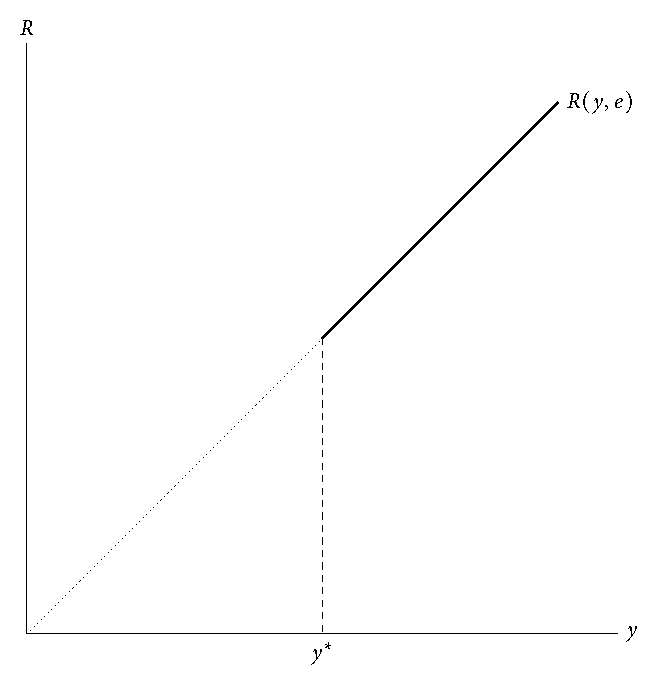
\includegraphics[width=0.7\textwidth]{optimal-R.pdf}
		\caption{The payment function $R(y,e)$. Before $y^*$ the physician is payed nothing and after $y^*$ the physician is the payed maximum of $R(y,e)$ }
		\label{fig:optimalPayRa}
	\end{figure}
				
	\begin{proof}
								
		Give \cref{eq:kt}  Lagrangian is
		\begin{align}
			\begin{split}                                                                    
			\mathcal{L}=[R(y,e)+\delta y]g(y|e)-C(e)+\mu [[R(y,e)+\delta y]g_e(y|e)-C_e(e)]+ \\ 
			\lambda [(y-R(y,e))g(y|e)-y_L^0]+\theta(y) R(y,e)+\theta(y)\left(y-R(y,e)\right) 
			\end{split}                                                                      
		\end{align}
		The first order conditions are
		\begin{subequations}
			\label{eq:foc}
			\begin{align}
				g(y|e)\left[1-\lambda+\mu \frac{g_e(y|e)}{g(y|e)}\right] +\theta(y)-\eta(y)                     & =0 \label{subeq:foc1} \\
				[R(y,e)+\delta y]g_e(y|e)-C_e(e)+\mu\left[[R(y,e)+\delta y]g_{ee}(y|e)- C_{ee(e)}\right] \qquad & \nonumber             \\ 
				+\lambda\left[(y-R(y,e)) g_e(y|e)-y_l^0\right]                                                  & =0 \label{subeq:foc2} 
			\end{align}
		\end{subequations}
		Because of non-negativity and complementary slackness conditions for $\theta(y)$ and $\eta(y)$, \cref{subeq:foc1} yields
		\begin{subequations}
			\label{eq:KT-analysis}
			\begin{alignat}{3}
				\phi(y,e) = g(y|e)\left[1-\lambda+\mu \frac{g_e(y|e)}{g(y|e)}\right]
				          & \: > \: & 0 & \enspace \Rightarrow &   & \enspace R(y,e)=y \label{subeq:large-y}           \\
				\phi(y,e) & \: = \: & 0 & \enspace \Rightarrow &   & \enspace R(y,e)\in [0,y] \label{subeq:interval-y} \\
				\phi(y,e) & \: < \: & 0 & \enspace \Rightarrow &   & \enspace R(y,e) =0 \label{subeq:small-y}          
			\end{alignat}
		\end{subequations}
								
		It is clear from \cref{subeq:foc1,eq:mlrp} that for $y$ large enough \cref{subeq:large-y} is always feasible. However, feasibility of \cref{subeq:interval-y,subeq:large-y} is not guaranteed, even for $y=0$ However, if $1>-\lambda+\mu \frac{g_e(y|e)}{g(y|e)}$, which is likely, then there must be some range of $e$ where \cref{subeq:large-y} (and thereby also \cref{subeq:interval-y}) holds. Thereby, as $\mu>0$ and the MLRP is increasing, $\phi(y,e)$ is also increasing.
								
		To prove (i) that $y=y_L^0$, note that the middle part of \cref{subeq:foc2} is strictly negative by \cref{asump:unique-solution}. Also note that by optimality, the first part is zero. I then follows that the last term must be strictly positive. As $\lambda\geq0$, $\lambda$ must be positive and by complementarity of slackness and so the hospitals participation constraint must bind. 
								
		to prove (ii), that the solution is below the \emph{first-best}, note that given (i) it is trivial that $y\in[0,y]$. Thereby I can write the optimal contract as 
		\[
			R(y,e)=\frac{1}{\lambda}+\frac{\mu}{\lambda}\frac{g_e(y_L^0|e)}{g(y_L^0|e)}>R_\lambda(y)
		\]
								
		To prove (iii), note when $\mu=0$, $R(y,e)=\frac{1}{\lambda}=R_\lambda(y)$
								
	\end{proof} 
	% subsection output_dependent_wage (end)
	% section optimal_payment_with_a_risk_neutral_agent (end)
	%\todo{Maybe write something about why $\delta y$ does not affect the solution}
	\section{Optimal payment with a risk averse agent} % (fold)
	\label{sec:optimal_payment_with_a_risk_averse_agent}
	I know introduce a risk averse agent with utility $u(R(y,e))$, such that $u'>0$ and $u''<0$. The problem is then restated as 
				
	\begin{subequations}
		\label{eq:ktRa}
		\begin{align}
			\max_{R,e}   & \int_0^{\infty}u(R(y,e))g(y|e)\dif y-C(e)\label{subeq:ktRa1}           \\
			\text{s.t. } & \int_{0}^{\infty} (y-R(y,e))g(y|e)\dif y\geq y_L^0 \label{subeq:ktRa2} \\
			             & E[u(R(y,e),y)|e]\leq E[u(R,e^*)|e] \label{subeq:ktRa3}                 \\
			             & 0\leq R(y,e)\leq y \label{subeq:ktRa4}                                 
		\end{align}
	\end{subequations}
				
	Using the first order approach as before I get that 
				
	\begin{subequations}
		\label{eq:lagrange-ra}
		\begin{align}
			u'(R(y,e))g(y|e)\left[1-\lambda+\mu \frac{g_e(y|e)}{g(y|e)}\right] + \theta(y)-\eta(y)=0             \\
			g_e(y|e)\left[(1+\mu)u(R(y,e))\frac{g_{ee}(y|e)}{g_e(y|e)}+\lambda(y-R(y,e))\right]-c_e(e)-c_{ee}(e) 
		\end{align}
	\end{subequations}
				
	Again define 
	\[
		\phi(y,e) = u'(R(y,e))g(y|e)\left[1-\lambda+\mu \frac{g_e(y|e)}{g(y|e)}\right]  + \theta(y)-\eta(y)
	\]
				
	\begin{subequations}
		\label{eq:KT-analysis-ra}
		\begin{alignat}{3}
			\phi(y,e) & \: > \: & 0 & \enspace \Rightarrow &   & \enspace R(y,e)=y \label{subeq:large-y-ra}           \\
			\phi(y,e) & \: = \: & 0 & \enspace \Rightarrow &   & \enspace R(y,e)\in [0,y] \label{subeq:interval-y-ra} \\
			\phi(y,e) & \: < \: & 0 & \enspace \Rightarrow &   & \enspace R(y,e) =0 \label{subeq:small-y-ra}          
		\end{alignat}
	\end{subequations}
				
	Further, by implicitly defining $R(y,e)\in[0,y]$ by 
	\[
		\frac{1}{u'(R(y,e))}=\frac{1}{\lambda}+\frac{\mu}{\lambda}\frac{g_e(y|e)}{g(y|e)}
	\]
	and noting that by concavity of $u(R(y,e))$, $R(y,e)$ is increasing in $e$. 
	%section optimal_payment_with_a_risk_averse_agent (end)
	\printbibliography%
	\listoftodos%
\end{document}